\minitoc
\newpage

\section*{Introduction}
\addcontentsline{toc}{section}{Introduction}

This sprint covers \textbf{Machine Monitoring, Production Order Management, and
  Operation History} in the \domainterm{MES} application, giving
\userrole{Operator}s and \userrole{Supervisor}s real-time visibility into machine
states and a full audit trail of completed operations.

It addresses three related sub-domains: live machine status tracking from
\techname{Business Central} to the \techname{Flutter} frontend, production order
management with operation lifecycle initiation, and a history view showing all
completed and cancelled operations per machine.

% ---------------------------------------------------------------------------
% 1. SPRINT BACKLOG
% ---------------------------------------------------------------------------
\section{Sprint Backlog}

This sprint covers \textbf{Domain 2:}
\textbf{\domainterm{Machine Monitoring, Production Order Management \& History}}.

% ----------------------------------------------------------
%  US-2.1
% ----------------------------------------------------------

% Guide: table captions ABOVE table; numbered as Section.Sequence
\begin{longtable}{@{} P{0.09\linewidth} P{0.34\linewidth} P{0.53\linewidth} @{}}
  \caption{Sprint Backlog}
  \label{tab:s2-sprint-backlog}\\
  \toprule
  \textbf{ID} & \textbf{User Story} & \textbf{Tasks} \\
  \midrule
  \endfirsthead
  \toprule
  \textbf{ID} & \textbf{User Story} & \textbf{Tasks} \\
  \midrule
  \endhead
  \multicolumn{3}{r}{\small Continued on next page} \\
  \endfoot
  \bottomrule
  \endlastfoot
  
  \textbf{US-2.1}
  & As an \userrole{Operator} or \userrole{Supervisor}, I need to see the list
  of machines in my work centre with their current status so that I can see
  which machines are currently active.
  & \noindent\textit{Business Central (AL):}
  \begin{itemize}[noitemsep, topsep=0pt, partopsep=0pt, leftmargin=*]
  \item Created table \techname{MES MachineStatus}.
  \item Created enum \techname{MES Machine Status}.
  \item Created function \texttt{FetchMachines()} in codeunit \techname{MES Machine Fetch}.
  \item Exposed \texttt{FetchMachines()} through codeunit \techname{MES Web Service}.
  \item Created page \techname{MES Machine List}.
  \end{itemize}
  \\ & &
  \noindent\textit{Flutter:}
  \begin{itemize}[noitemsep, topsep=0pt, partopsep=0pt, leftmargin=*]
  \item Created model \techname{MachineModel}.
  \item Created service \techname{MESMachineListService} to consume the \texttt{FetchMachines()} API.
  \item Created provider \techname{MesMachinesProvider}.
  \item Created page \techname{MachineListPage}.
  \item Created widget \techname{MachineCard}.
  \item Implemented automatic machine list refresh in \techname{MESMachineListService}.
  \end{itemize}\\
  \midrule
  \textbf{US-2.2}
  & As an \userrole{Operator} or \userrole{Supervisor}, I need to view the
  production orders assigned to a machine so that I know what work needs
  to be done.
  & \noindent\textit{Business Central (AL):}
  \begin{itemize}[noitemsep, topsep=0pt, partopsep=0pt, leftmargin=*]
    \item Created function \texttt{getMachineOrders()} in codeunit \techname{MES Machine Fetch}.
    \item exposed  \texttt{getMachineOrders()} in codeunit \techname{MES Web Service}.
  \end{itemize}
\\ & &
  \noindent\textit{Flutter:}
  \begin{itemize}[noitemsep, topsep=0pt, partopsep=0pt, leftmargin=*]
    \item Created model \techname{MachineOrderModel}.
    \item Created service \techname{ErpMachineOrdersService} to consume the \texttt{getMachineOrders()} API.
    \item Created provider \techname{MachineordersProvider}.
    \item Created page \techname{MachineOrderPage}.
    \item Created widget \techname{OrderCard}.
    \item Created model \techname{BadgeStyle}.
  \end{itemize}\\
  \midrule
  \textbf{US-2.3}
  & As an \userrole{Operator} or \userrole{Supervisor}, I need to start a
  production operation so that the system records that the order has begun.
  & \noindent\textit{Business Central (AL):}
  \begin{itemize}[noitemsep, topsep=0pt, partopsep=0pt, leftmargin=*]
    \item Created table \techname{MES Operation state}.
    \item Created enum \techname{MES Operation Status}.
    \item Created function \texttt{TryStartOperation()} in codeunit \techname{MES Machine Validation}.
    \item Created function \texttt{InsertMESOperation()} in codeunit \techname{MES Machine Write}.
    \item Exposed \texttt{InsertMESOperation()} through codeunit \techname{MES Web Service}.
    \item Created page \techname{MES Operations}.
  \end{itemize}

  \noindent\textit{Flutter:}
  \begin{itemize}[noitemsep, topsep=0pt, partopsep=0pt, leftmargin=*]
    \item Implemented \techname{ErpMachineOrdersService} that Consumes the \texttt{startOperation} API.
    \item Implement \techname{MachineordersProvider} to manage its state.
    \item Implemented start operation action handling in \techname{ActionButtons}.
    \item Implemented automatic navigation to \techname{OrdersProgressionPage}
  \end{itemize}\\
  \midrule
  \textbf{US-2.4}
  & As a \userrole{Supervisor} or \userrole{Operator}, I need to monitor the
  current status of all active operations on a machine so that I can follow
  the progress of each order.
  & \noindent\textit{Business Central (AL):}
  \begin{itemize}[noitemsep, topsep=0pt, partopsep=0pt, leftmargin=*]
    \item Created function \texttt{fetchMachineOperationStatus()} in codeunit \techname{MES Machine Fetch}.
    \item Exposed \texttt{fetchMachineOperationStatus()} through codeunit \techname{MES Web Service}.
  \end{itemize}
\\ & &
  \noindent\textit{Flutter:}
  \begin{itemize}[noitemsep, topsep=0pt, partopsep=0pt, leftmargin=*]
    \item Updated \techname{ErpMachineOrdersService}to Consume the \texttt{fetchMachineOperationStatus}.
    \item Created model \techname{OperationStatusStyle}.
    \item Created page \techname{OrdersProgressionPage}.
    \item Created the widgets \techname{OperationCard}, \techname{OperationStatusBadge}, widget \techname{OperationInfoGrid}, and \techname{OperationProgressBar}.
    \item Implemented automatic refresh for operation status monitoring.
  \end{itemize} \\
  \midrule
  \textbf{US-2.5}
  & As an \userrole{Operator} or \userrole{Supervisor}, I need a tabbed view
  for a machine so that I can navigate between pending orders and active
  operation progress without leaving the machine context.
  & \noindent\textit{Flutter:}
  \begin{itemize}[noitemsep, topsep=0pt, partopsep=0pt, leftmargin=*]
    \item Created page \techname{MachineMainPage}.
    \item Created the widgets \techname{TopNavigationBar} and \techname{NavButton}.
    \item Implemented tab navigation in \techname{MachineMainPage}.
    \item Implemented navigation from \techname{MachineCard} to \techname{MachineMainPage}.
  \end{itemize} \\
  \midrule
  \textbf{US-2.6}
  & As an \userrole{Operator} or \userrole{Supervisor}, I need to filter and
  sort production orders so that I can quickly find the most relevant work.
  & \noindent\textit{Flutter:}
  \begin{itemize}[noitemsep, topsep=0pt, partopsep=0pt, leftmargin=*]
    \item Created widget \techname{GlobalSearchBar}.
    \item Implemented order search, filtering, and sorting in \techname{MachineOrderPage}.
  \end{itemize} \\
  \midrule
  \textbf{US-2.7}
  & As a \userrole{Supervisor} or \userrole{Operator}, I need to view the
  history of completed operations for a machine so that I can audit past
  production.
  & \noindent\textit{Business Central (AL):}
  \begin{itemize}[noitemsep, topsep=0pt, partopsep=0pt, leftmargin=*]
    \item Created function \texttt{fetchOperationsStatusAndProgress()} in codeunit \techname{MES Machine Fetch}.
    \item Exposed \texttt{fetchOperationsStatusAndProgress()} in codeunit \techname{MES Web Service}.
  \end{itemize}
\\ & &
  \noindent\textit{Flutter:}
  \begin{itemize}[noitemsep, topsep=0pt, partopsep=0pt, leftmargin=*]
    \item Updated \techname{ErpMachineOrdersService} to consume the \texttt{fetchMachineOperationStatusAndProgress} API.
    \item Updated \techname{MachineordersProvider} to manage its state.
    \item Created page \techname{MachineHistoryPage}.
    \item Created the widgets \techname{HistoryCard}, \techname{HistoryBadgeAndId}, and \techname{HistoryInfoGrid}.
    \item Implemented history search and sorting in \techname{MachineHistoryPage}.
    \item Implemented navigation from \techname{HistoryCard} to \techname{OperationDetailPage}.
  \end{itemize}\\  
\end{longtable}

% ---------------------------------------------------------------------------
% 2. BUSINESS RULES
% ---------------------------------------------------------------------------
\section{Business Rules}

\Needspace{12\baselineskip}
\begin{longtable}{@{} P{0.30\linewidth} P{0.65\linewidth} @{}}
	\caption{Business Rules}
	\label{tab:s2-Business-Rules}\\
	\toprule
	\textbf{ID: Business Rule} & \textbf{Description} \\
	\midrule
	\endfirsthead
	\toprule
	\textbf{ID: Business Rule} & \textbf{Description} \\
	\midrule
	\endhead
	\multicolumn{2}{r}{\small Continued on next page} \\
	\endfoot
	\bottomrule
	\endlastfoot
	
	\multicolumn{2}{@{}l}{\textbf{Machine Status Rules}} \\
	\midrule
	
	\businessrule{BR-MCH-001}: Machine Status Tracking &
	\begin{itemize}
	  \item Machine status is stored as an append-only log in the
	        \modulename{MES Machine Status} table; the latest record per machine
	        represents the current state.
	  \item Valid statuses are \domainterm{Idle}, \domainterm{Starting}, and
	        \domainterm{OutOfOrder}.
	  \item The \techname{Flutter} frontend polls the status endpoint every 5 seconds
	        via a \domainterm{Stream} to maintain a live view.
	\end{itemize} \\
	\midrule
	
	\businessrule{BR-MCH-002}: Work Centre Scoping &
	\begin{itemize}
	  \item The machine list is always filtered to the work centre stored in the
	        authenticated user's session token response.
	  \item An \userrole{Operator} or \userrole{Supervisor} can only see machines
	        belonging to their assigned work centre.
	\end{itemize} \\
	\midrule
	
	\multicolumn{2}{@{}l}{\textbf{Operation Lifecycle Rules}} \\
	\midrule
	
	\businessrule{BR-OPS-001}: Start Operation Validation &
	\begin{itemize}
	  \item Only routing lines with status \domainterm{Released} may be started.
	  \item An operation that already has a \domainterm{Running} record may not be
	        started again.
	  \item A machine may not run more than one operation at a time; attempting to
	        start a second operation on a busy machine is rejected with a descriptive
	        error message.
	\end{itemize} \\
	\midrule
	
	\businessrule{BR-OPS-002}: Immutable Operation History &
	\begin{itemize}
	  \item Each state transition (start, pause, resume) inserts a \emph{new} record
	        into \modulename{MES Operation Status} rather than modifying an existing
	        one, preserving a full audit trail.
	  \item The latest status for a given (machine, order, operation) triple is
	        determined by sorting on \modulename{Last Updated At} descending and
	        taking the first record.
	\end{itemize} \\
	\midrule
	
	\businessrule{BR-OPS-003}: Active Operation Query &
	\begin{itemize}
	  \item When fetching active operations for a machine, the backend groups records
	        by (production order, operation) and returns only those whose most recent
	        record has status \domainterm{Running} or \domainterm{Paused}.
	  \item Operations whose latest record is \domainterm{Finished} are excluded from
	        the active list.
	\end{itemize} \\
	\midrule
	
	\multicolumn{2}{@{}l}{\textbf{History Query Rules}} \\
	\midrule
	
	\businessrule{BR-HIST-001}: History Scope &
	\begin{itemize}
	  \item The History tab queries \modulename{fetchOperationsStatusAndProgress}
	        with \texttt{fetchFinished = true}, returning only \domainterm{Finished}
	        and \domainterm{Cancelled} executions.
	  \item The earliest \domainterm{Running} status timestamp is resolved as
	        \texttt{startDateTime}; the first \domainterm{Finished} or
	        \domainterm{Cancelled} timestamp as \texttt{endDateTime}.
	  \item History is loaded as a one-shot \texttt{Future} on page open; it is
	        not polled, as completed records are immutable.
	\end{itemize} \\
\end{longtable}

% ---------------------------------------------------------------------------
% 3. DESIGN
% ---------------------------------------------------------------------------
\section{Design}


\subsection{Use Case Diagram}

\begin{figure}[H]
  \centering
  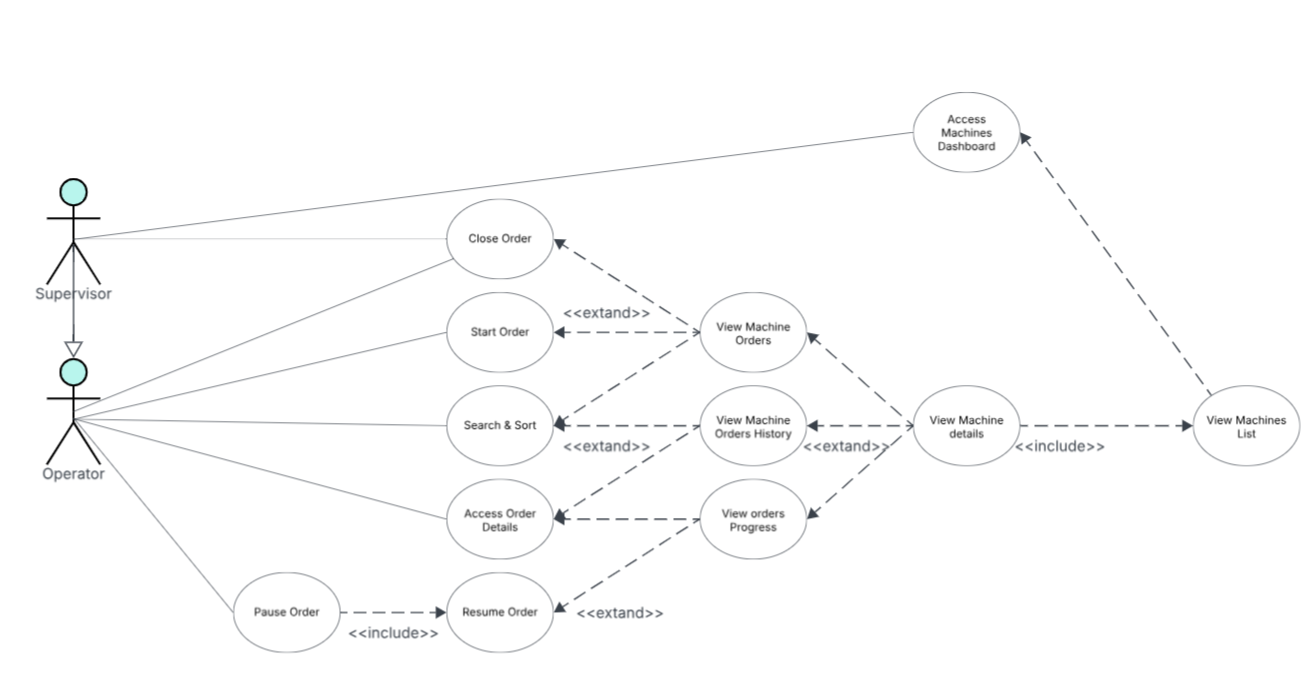
\includegraphics[width=6in]{./media/MES_Sprint-2-Repport/diagrams/useCase/sprint2.png}
  \caption{UML Use Case Diagram --- Machine \& Production Management.}
  \label{fig:s2-use-case-diagram-s2}
\end{figure}


The UML Use Case Diagram (Figure~\ref{fig:s2-use-case-diagram-s2}) shows the two
primary actors (\userrole{Operator} and \userrole{Supervisor}) and their
interactions with the machine monitoring, production order management, and history
subsystem. In addition to viewing machines, browsing orders, and managing operation
lifecycle transitions, the diagram includes the \uilabel{View Operation History}
use case, which allows both actors to access the completed and cancelled operation
log for any machine in their work centre.

\subsection{Textual Use Case Description}

The following table (Table~\ref{tab:s2-use-case-start-operation}) provides the detailed
textual description of the \textit{Start Operation} use case.

\Needspace{10\baselineskip}
\begin{longtable}{@{} P{0.21\linewidth} P{0.75\linewidth} @{}}
  
  \caption{Textual Use Case Description --- Start Operation}
  \label{tab:s2-use-case-start-operation}\\
  \toprule
  \endfirsthead
  
  \midrule
  \endhead
  
  \midrule
  \multicolumn{2}{r}{\small Continued on next page}\\
  \endfoot
  
  \bottomrule
  \endlastfoot
  
  \textbf{Use Case Name}  & Start Operation     \\
  \midrule
  \textbf{Primary Actor}  & \userrole{Operator} \\
  \midrule
  \textbf{Preconditions}  &                     
  \begin{itemize}[noitemsep, topsep=0pt, partopsep=0pt, leftmargin=*]
  \item The \userrole{Operator} is authenticated and has a valid session token.
  \item The target routing line has status \domainterm{Released}.
  \item No other operation is currently \domainterm{Running} on the same machine.
  \item The operation has not already been started (no existing
  \domainterm{Running} record for this order/operation pair).
  \end{itemize} \\
  \midrule
  
  \textbf{Postconditions} &                     
  \begin{itemize}[noitemsep, topsep=0pt, partopsep=0pt, leftmargin=*]
  \item A new \modulename{MES Operation Status} record is inserted with status
  \domainterm{Running} and the current \domainterm{UTC} timestamp.
  \item The \uilabel{Operations Progress} tab reflects the new running operation
  within the next polling cycle.
  \item If any precondition fails, a descriptive error dialog is shown to the
  operator and no record is inserted.
  \end{itemize} \\
  \midrule
  
  \textbf{Main Scenario}  &                     
  \begin{enumerate}[noitemsep, topsep=0pt, partopsep=0pt, leftmargin=*]
  \item The \userrole{Operator} navigates to the \uilabel{Machine List Page} and
  selects a machine.
  \item The system displays the \uilabel{Machine Orders Page} listing all
  applicable production orders.
  \item The \userrole{Operator} locates a \domainterm{Released} order and taps
  \uilabel{Start Order}.
  \item The frontend sends a \domainterm{POST} request to
  \apiendpoint{MESMachinesActionsEndpoints\_startOperation}.
  \item The backend validates all preconditions (\businessrule{BR-OPS-001}).
  \item On success, a \modulename{MES Operation Status} record is inserted.
  \item The frontend navigates to the \uilabel{Orders Progression Page}.
  \end{enumerate} \\
  
\end{longtable}

\subsection{Sequence Diagrams}

The following sequence diagrams illustrate the communication flow between the
\techname{Flutter} frontend, the \techname{Business Central} OData layer, and the
\techname{AL} business logic for each machine and operation flow.

Figure~\ref{fig:s2-seq-fetch-machines} shows the fetch machines flow.
Figure~\ref{fig:s2-seq-machine-orders} illustrates the get machine orders flow.
Figure~\ref{fig:s2-seq-start-operation} depicts the start operation flow.
Figure~\ref{fig:s2-seq-fetch-ops-status} presents the fetch operations status flow.

\begin{figure}[H]
  \centering
  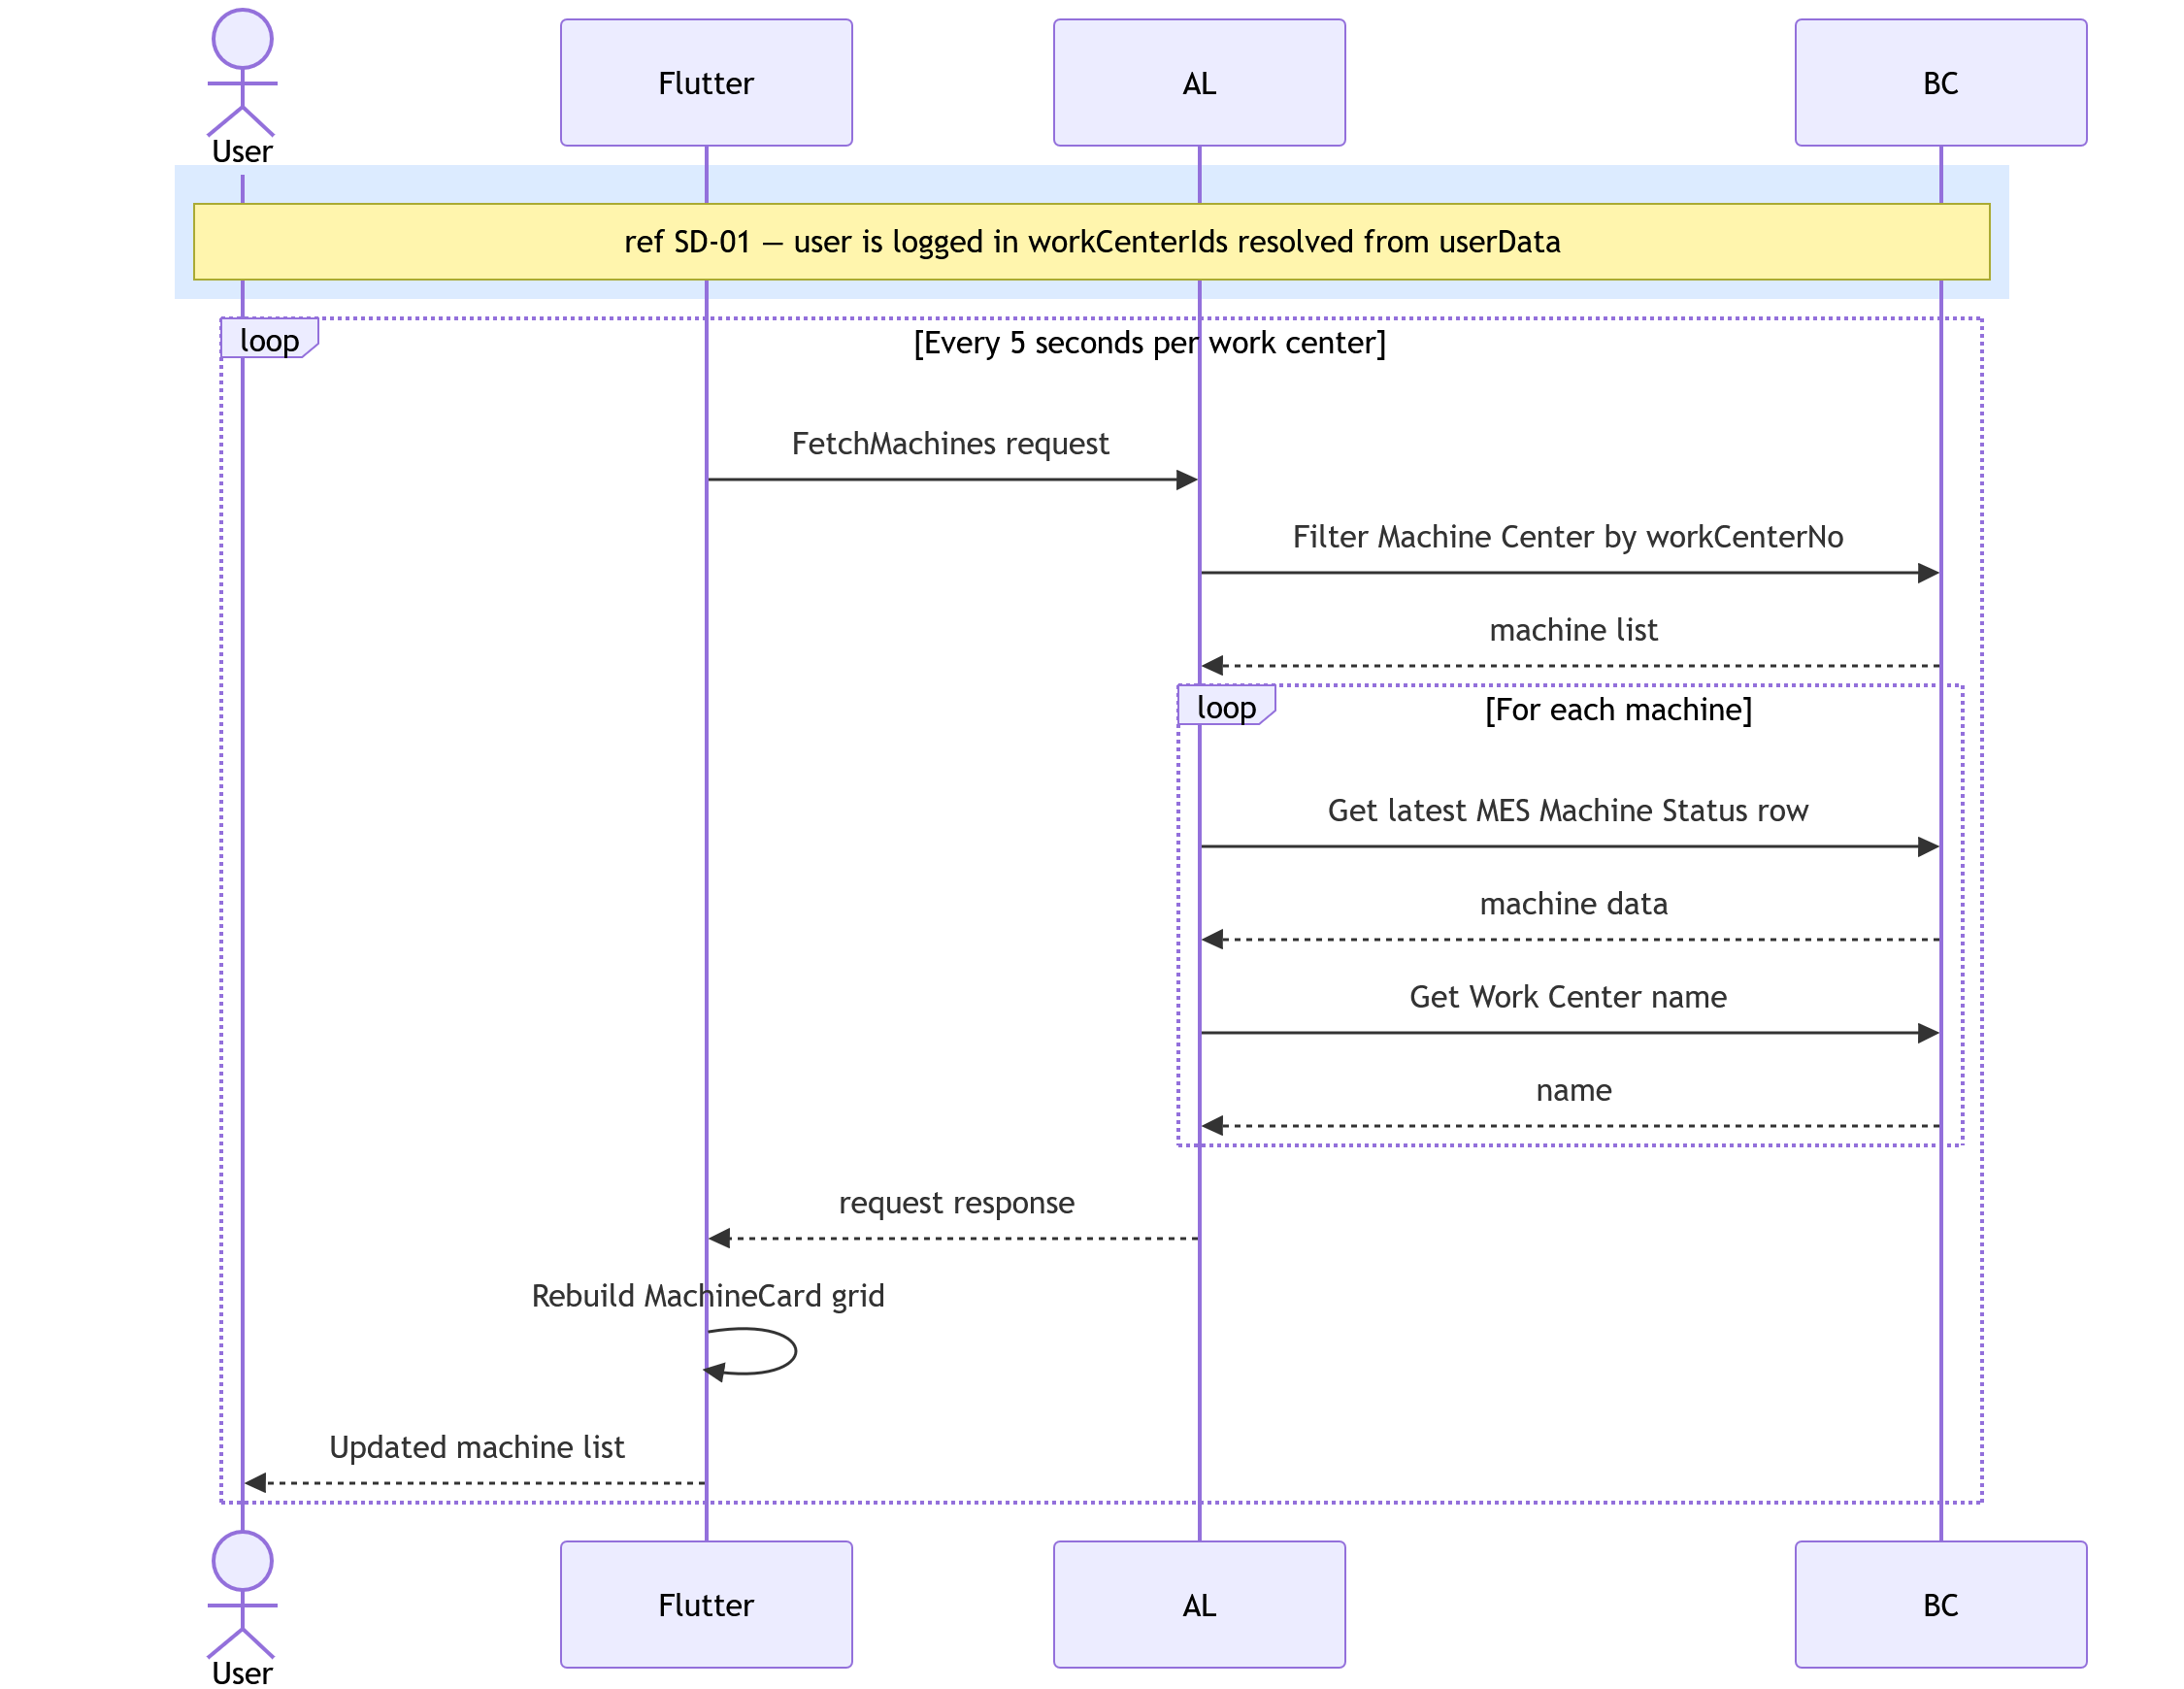
\includegraphics[width=\linewidth,keepaspectratio]{./media/MES_Sprint-2-Repport/diagrams/sequence/fetch-machines.png}
  \caption{SD-09: Fetch Machines.}
  \label{fig:s2-seq-fetch-machines}
\end{figure}

%=====SD-09==========================================================
% sequenceDiagram
%     actor User
%     participant Flutter
%     participant AL
%     participant BC

%     rect rgb(220,235,255)
%         Note over User,BC: ref SD-01 — user is logged in workCenterIds resolved from userData;
%     end

%     loop Every 5 seconds per work center
%         Flutter->>AL: FetchMachines request
%         AL->>BC: Filter Machine Center by workCenterNo
%         BC-->>AL: machine list
%         loop For each machine
%             AL->>BC: Get latest MES Machine Status row
%             BC-->>AL: machine data
%             AL->>BC: Get Work Center name
%             BC-->>AL: name
%         end
%         AL-->>Flutter: request response
%         Flutter->>Flutter: Rebuild MachineCard grid
%         Flutter-->>User: Updated machine list
%     end
%====================================================================

\begin{figure}[H]
  \centering
  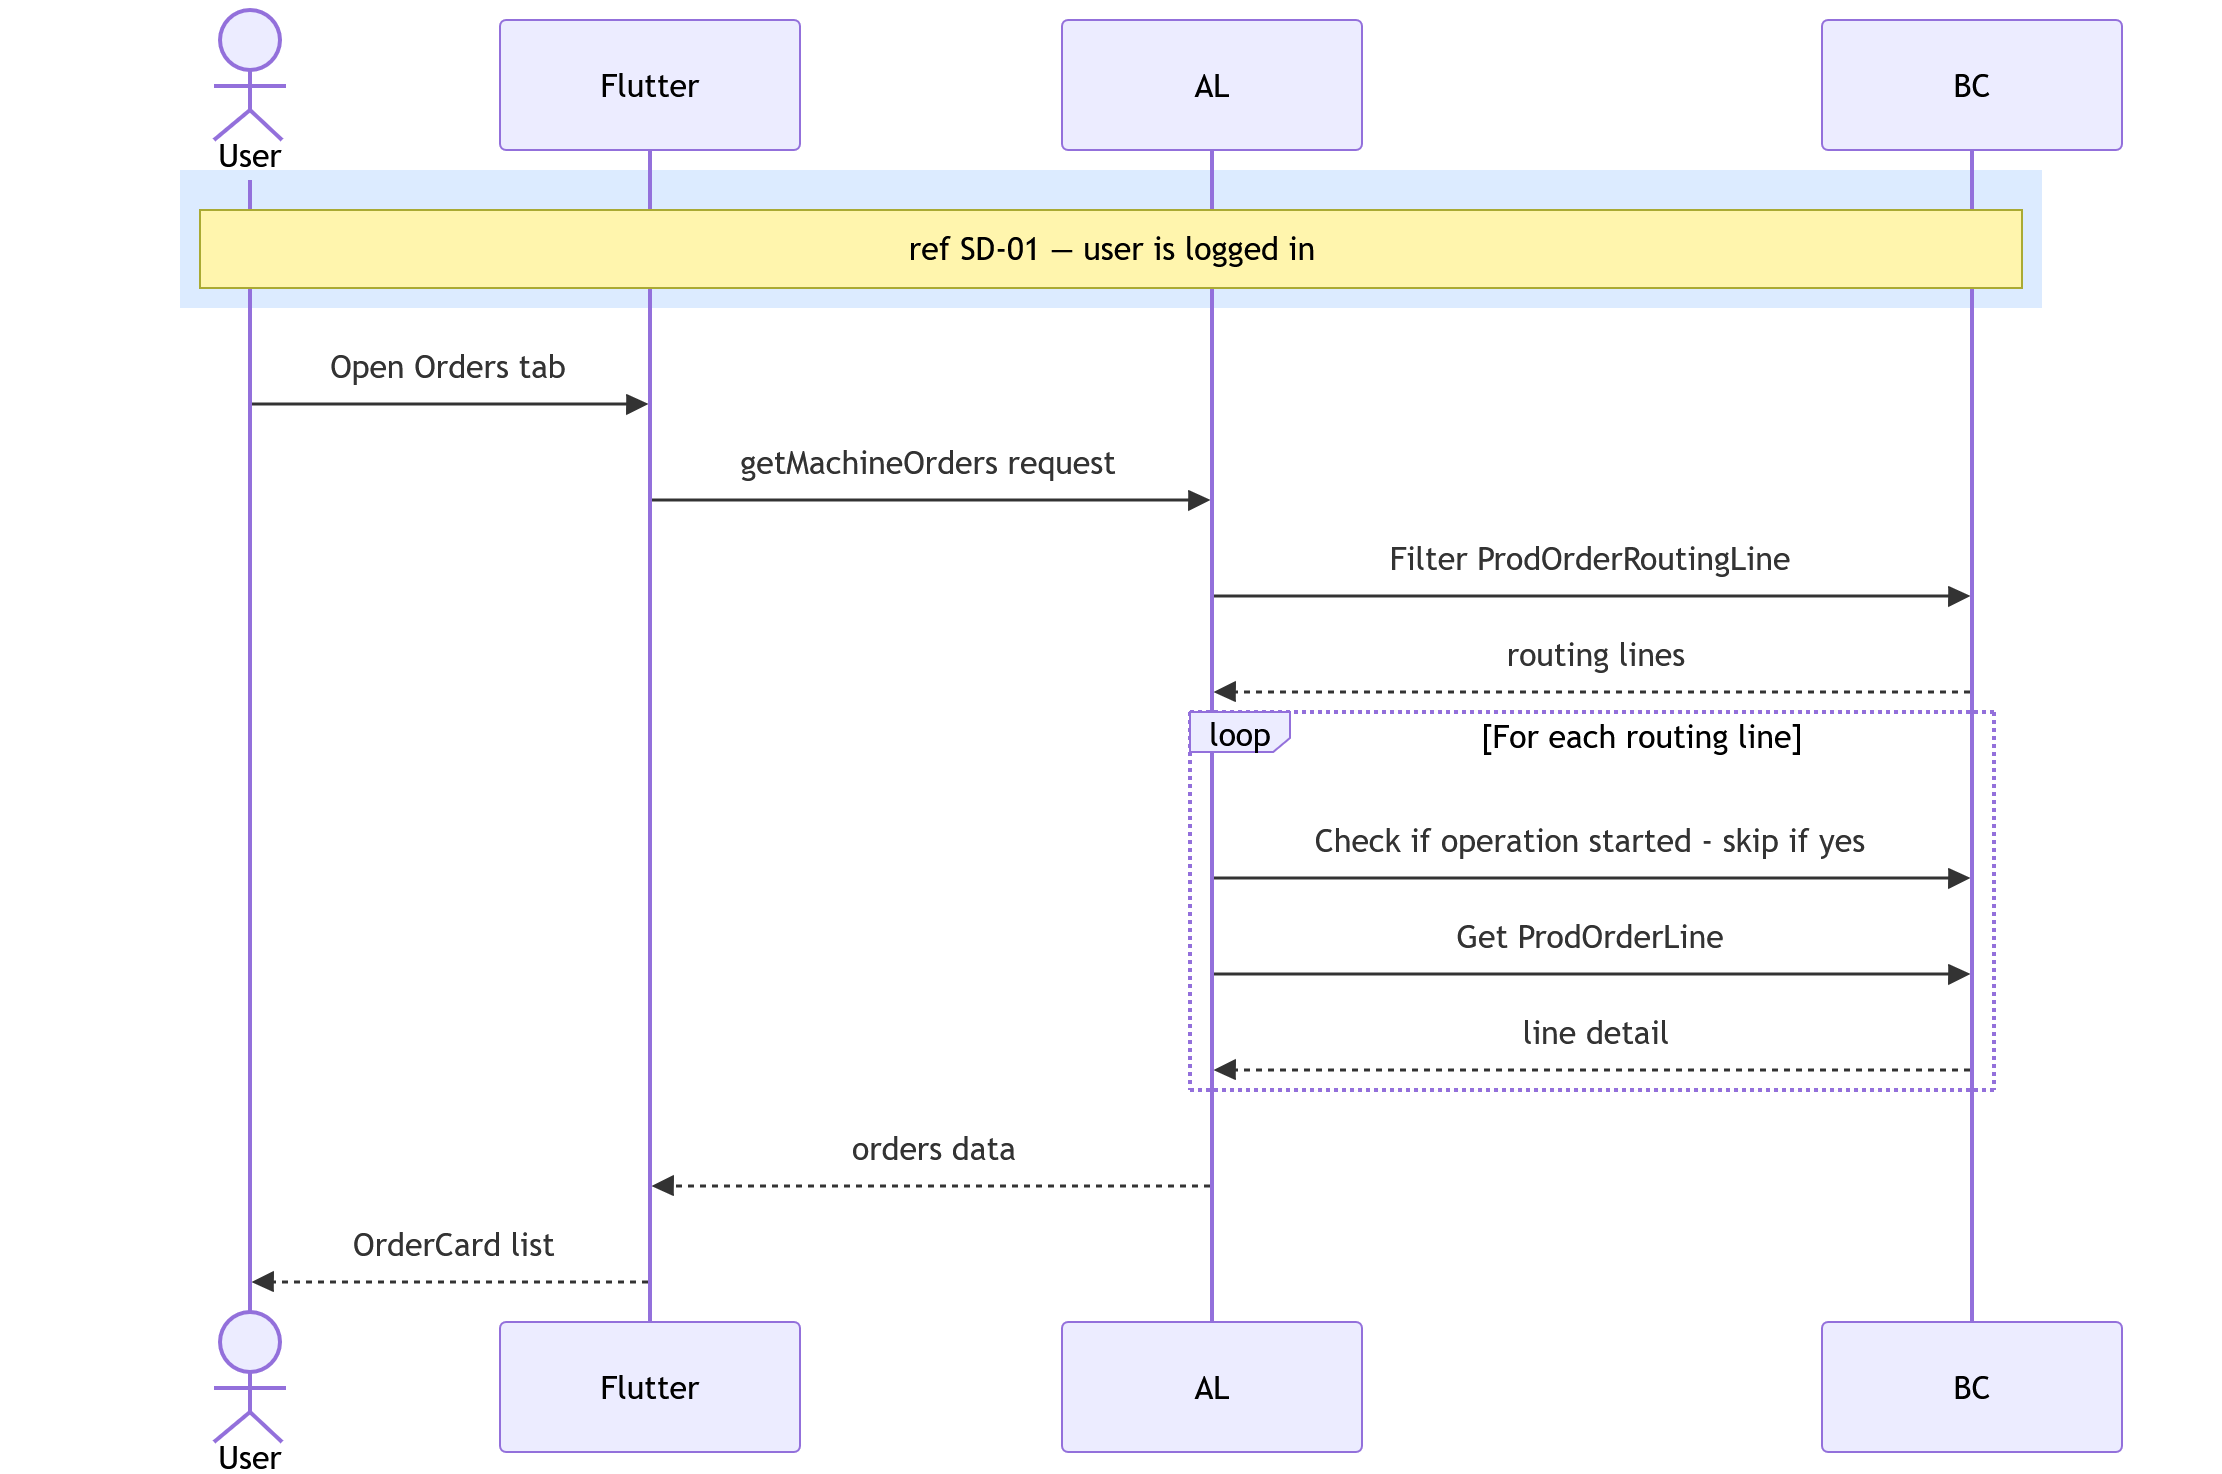
\includegraphics[width=\linewidth,keepaspectratio]{./media/MES_Sprint-2-Repport/diagrams/sequence/waiting-orders.png}
  \caption{SD-10: Get Machine Orders.}
  \label{fig:s2-seq-machine-orders}
\end{figure}

%=====SD-10==========================================================
% sequenceDiagram
%     actor User
%     participant Flutter
%     participant AL
%     participant BC

%     rect rgb(220,235,255)
%         Note over User,BC: ref SD-01 — user is logged in
%     end

%     User->>Flutter: Open Orders tab
%     Flutter->>AL: getMachineOrders request
%     AL->>BC: Filter ProdOrderRoutingLine
%     BC-->>AL: routing lines
%     loop For each routing line
%         AL->>BC: Check if operation started - skip if yes
%         AL->>BC: Get ProdOrderLine
%         BC-->>AL: line detail
%     end
%     AL-->>Flutter: orders data
%     Flutter-->>User: OrderCard list
%====================================================================

\begin{figure}[H]
  \centering
  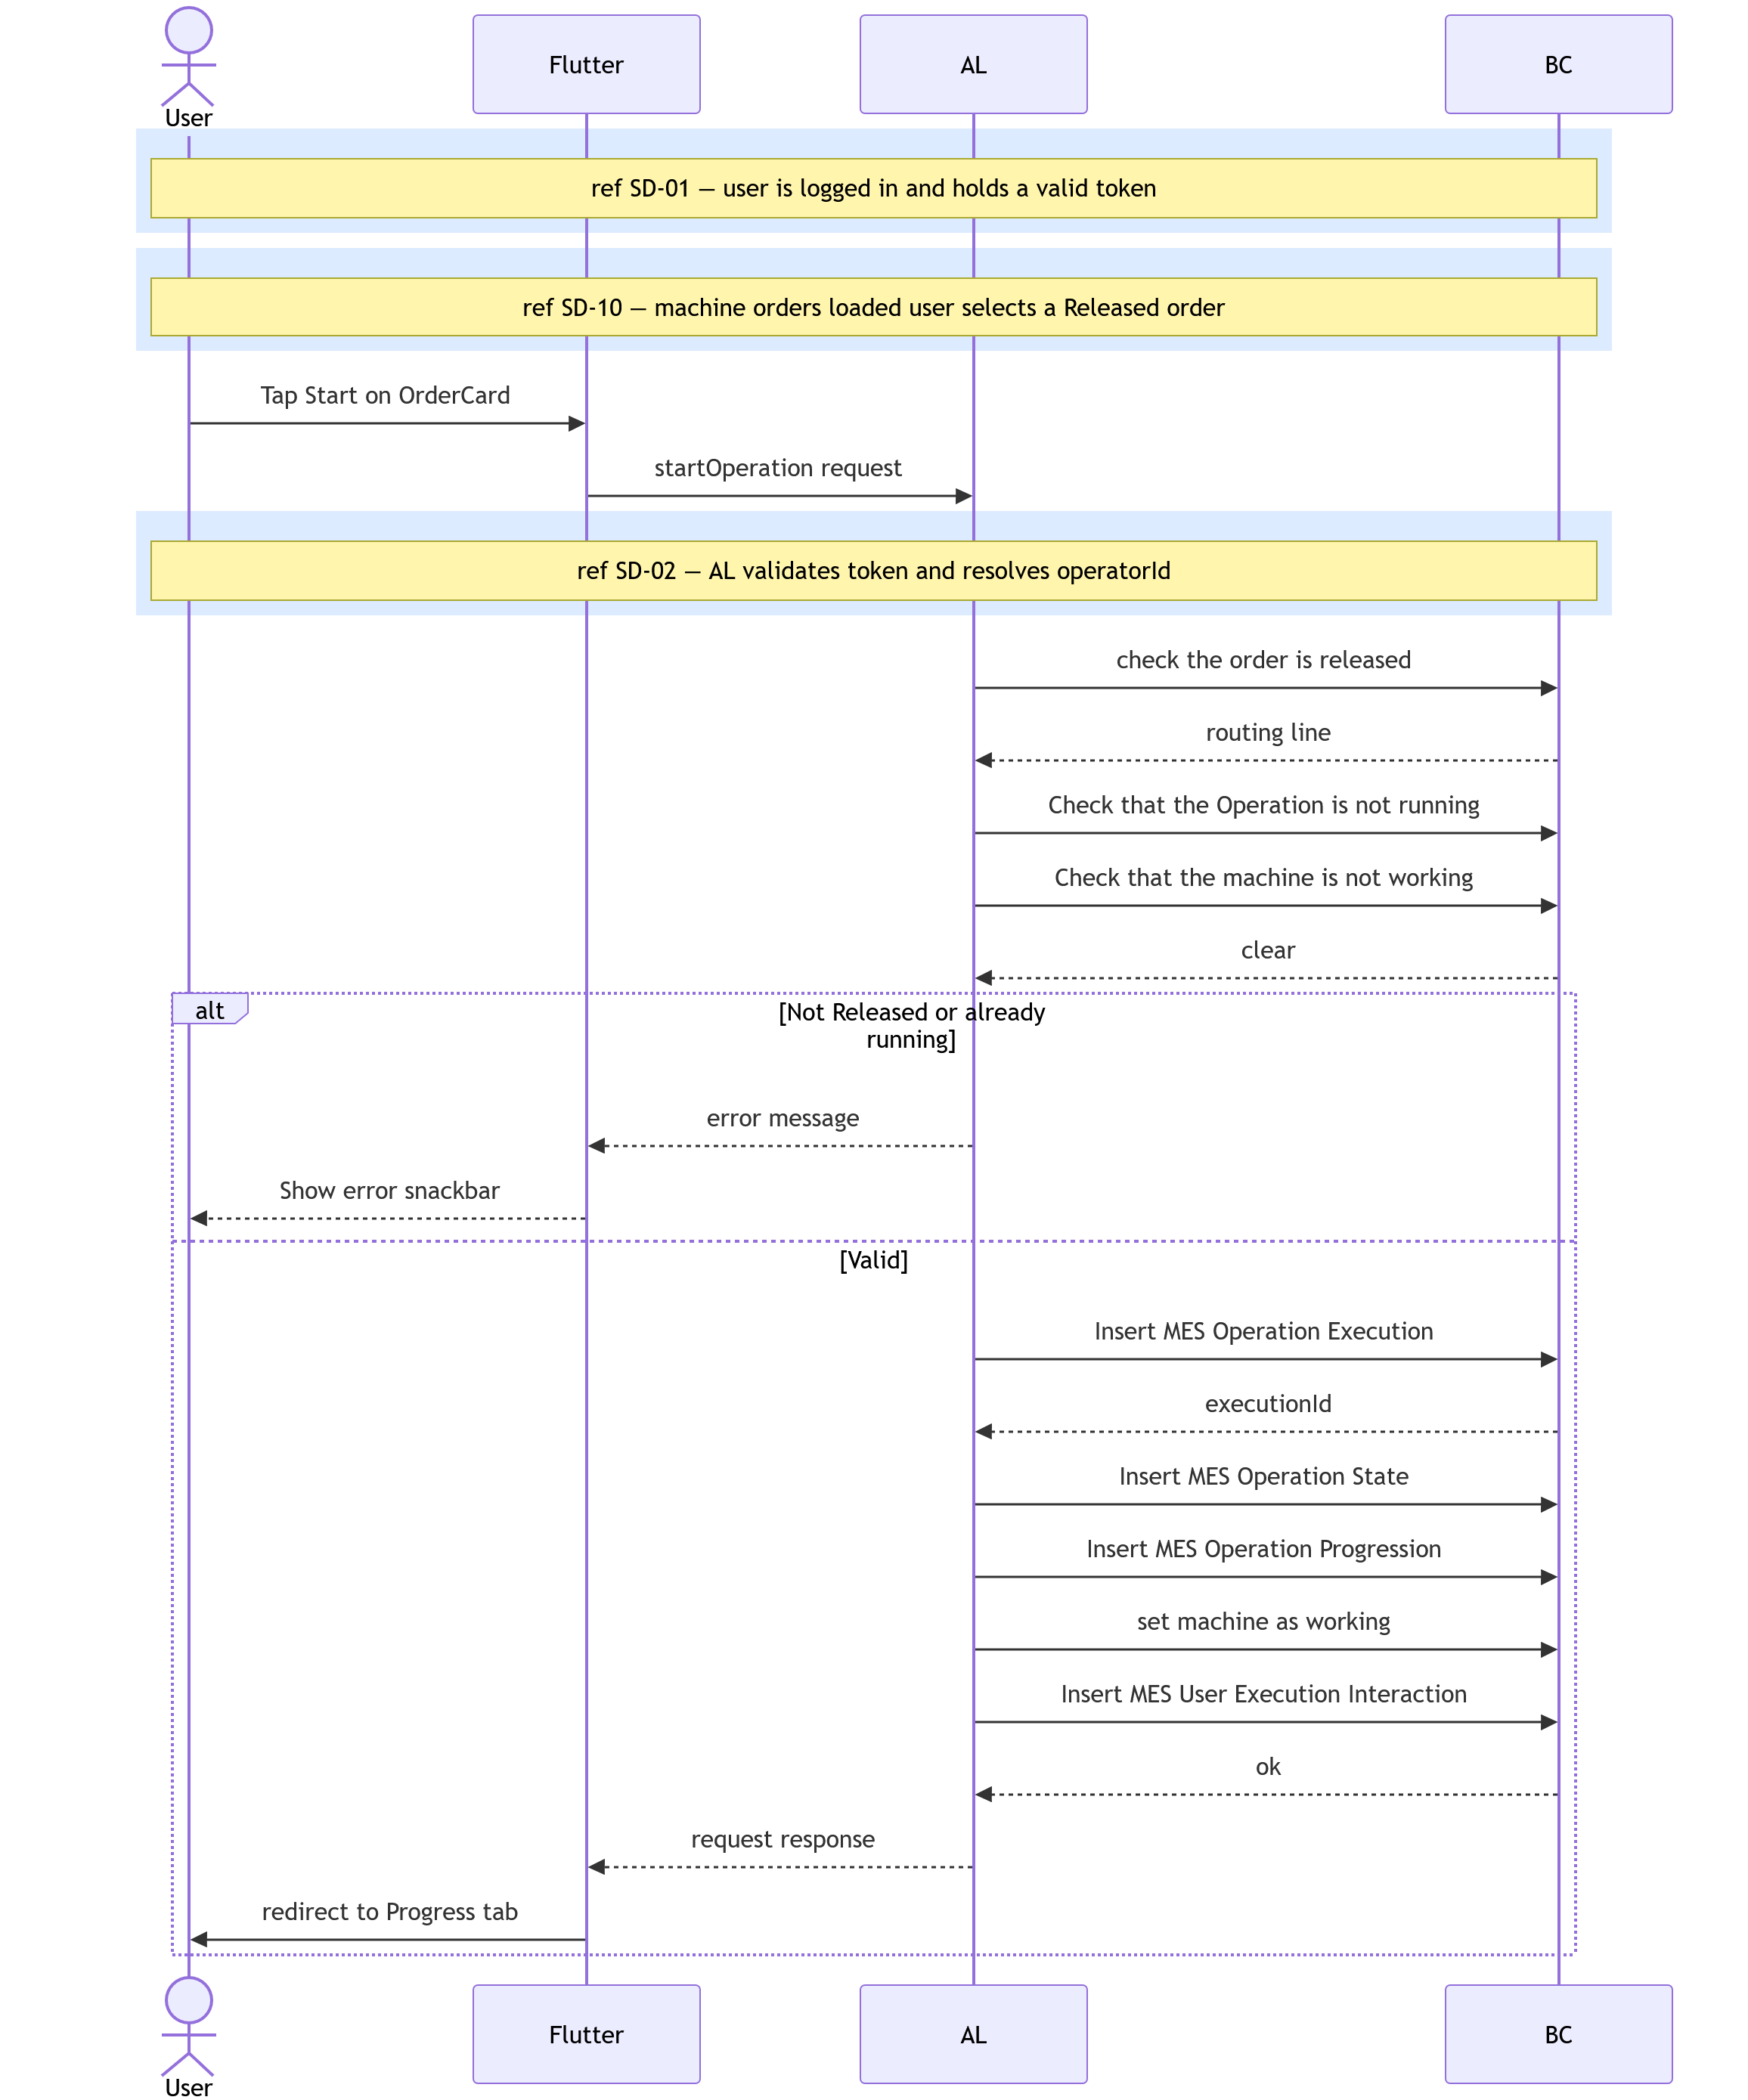
\includegraphics[width=\linewidth,height=0.82\textheight,keepaspectratio]{./media/MES_Sprint-2-Repport/diagrams/sequence/start-order.png}
  \caption{SD-11: Start Operation.}
  \label{fig:s2-seq-start-operation}
\end{figure}


%=====SD-11==========================================================
% sequenceDiagram
%     actor User
%     participant Flutter
%     participant AL
%     participant BC

%     rect rgb(220,235,255)
%         Note over User,BC: ref SD-01 — user is logged in and holds a valid token
%     end
%     rect rgb(220,235,255)
%         Note over User,BC: ref SD-10 — machine orders loaded user selects a Released order
%     end

%     User->>Flutter: Tap Start on OrderCard
%     Flutter->>AL: startOperation request

%     rect rgb(220,235,255)
%         Note over User,BC: ref SD-02 — AL validates token and resolves operatorId
%     end

%     AL->>BC: check the order is released
%     BC-->>AL: routing line
%     AL->>BC: Check that the Operation is not running
%     AL->>BC: Check that the machine is not working
%     BC-->>AL: clear
%     alt Not Released or already running
%         AL-->>Flutter: error message
%         Flutter-->>User: Show error snackbar
%     else Valid
%         AL->>BC: Insert MES Operation Execution
%         BC-->>AL: executionId
%         AL->>BC: Insert MES Operation State
%         AL->>BC: Insert MES Operation Progression
%         AL->>BC: set machine as working
%         AL->>BC: Insert MES User Execution Interaction
%         BC-->>AL: ok
%         AL-->>Flutter: request response
%         Flutter->>User: redirect to Progress tab
%     end
%====================================================================

\begin{figure}[H]
  \centering
  
\includegraphics[height=0.30\textheight,keepaspectratio]{./media/MES_Sprint-2-Repport/placeholder-image.png}
  \caption{Fetch Operation progress --- Sequence Diagram.}
  \label{fig:s2-seq-fetch-progress}
\end{figure}

\begin{figure}[H]
  \centering
  
\includegraphics[height=0.30\textheight,keepaspectratio]{./media/MES_Sprint-2-Repport/placeholder-image.png}
  \caption{Fetch Operation History --- Sequence Diagram.}
  \label{fig:s2-seq-fetch-history}
\end{figure}

Figure~\ref{fig:s2-seq-fetch-history} shows the history retrieval sequence. The
\techname{Flutter} frontend calls the same
\apiendpoint{fetchOperationsStatusAndProgress} endpoint used by the active
monitoring view, but with \texttt{fetchFinished = true}. The
\techname{Business Central} backend returns only executions whose latest status
record is \domainterm{Finished} or \domainterm{Cancelled}, along with resolved
start and end timestamps.

\subsection{Class Diagram}

The UML Class Diagram (Figure~\ref{fig:s2-class-diagram-s2}) of the machine and
production management domain shows the \modulename{MES Machine Status} and
\modulename{MES Operation Status} tables and their relationships with the
\techname{Business Central} standard tables \modulename{Machine Center} and
\modulename{Prod. Order Routing Line}.

\begin{figure}[H]
  \centering
  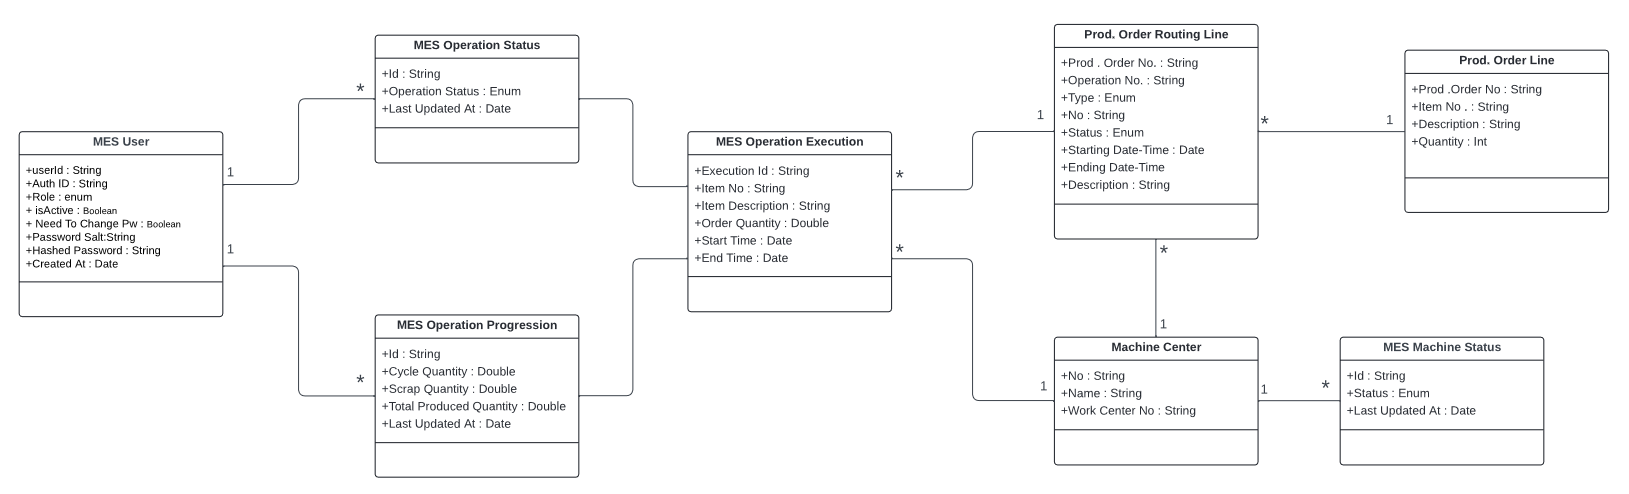
\includegraphics[width=\linewidth,height=0.82\textheight,keepaspectratio]{./media/MES_Sprint-2-Repport/diagrams/class/sprint2-diagram.png}
  \caption{UML Class Diagram --- Machine \& Production Management.}
  \label{fig:s2-class-diagram-s2}
\end{figure}

% ---------------------------------------------------------------------------
% 4. IMPLEMENTATION
% ---------------------------------------------------------------------------
\section{Implementation}

\subsection{Backend Implementation}

\subsubsection{Backend Structure Overview}

The machines domain follows the same layered structure established in Sprint~1.
Two new sub-folders were added under \modulename{src/1-Tables/machines/} and
\modulename{src/2-Enum/machines/}, and a new codeunit was placed under
\modulename{src/3-CodeUnit/machines/}. The OData web service is published through
the existing \modulename{WebServices.xml} mechanism under a new service name.

\subsubsection{MES Machine Status Table}

The \modulename{MES Machine Status} table (50107) stores the full history of
machine state changes as an append-only log. Each insert creates a new record;
the most recent record per machine represents the current state. Table~\ref{tab:s2-mes_machine_status_fields}
lists the fields and their descriptions.

\begin{longtable}{@{} P{0.21\linewidth} P{0.17\linewidth} P{0.57\linewidth} @{}}
  
  \caption{MES Machine Status (Table 50107) --- Field Dictionary}
  \label{tab:s2-mes_machine_status_fields}\\
  \toprule
  \textbf{Name}           & \textbf{Type}                      & \textbf{Description} \\
  \midrule
  \endfirsthead
  
  \toprule
  \textbf{Name}           & \textbf{Type}                      & \textbf{Description} \\
  \midrule
  \endhead
  
  \multicolumn{3}{r}{\small Continued on next page} \\
  \endfoot
  
  \bottomrule
  \endlastfoot
  
  Id                      & Code[50]                           &                      
  Primary key. GUID-derived value assigned automatically on insert if blank. \\
  \midrule
  
  Machine No.             & Code[20]                           &                      
  Foreign key to \texttt{Machine Center."No."}. Identifies the machine this status
  record belongs to. \\
  \midrule
  
  Status                  & Enum (\texttt{MES Machine Status}) &                      
  Current machine state: \domainterm{Idle}, \domainterm{Starting}, or
  \domainterm{OutOfOrder}. \\
  \midrule
  
  Current Prod. Order No. & Code[20]                           &                      
  Foreign key to \texttt{Prod. Order Routing Line."Prod. Order No."}. Records which
  production order the machine is currently executing, if any. \\
  \midrule
  
  Last Updated At         & DateTime                           &                      
  UTC timestamp set automatically on insert. Used to find the most recent status
  record for a given machine. \\
  
\end{longtable}

\subsubsection{MES Operation Status Table}

The \modulename{MES Operation Status} table (50108) implements the same
append-only pattern for operation lifecycle events. Every state transition
(start, pause, resume, finish) inserts a new record; queries always sort by
\modulename{Last Updated At} descending to obtain the current state.
Table~\ref{tab:s2-mes_operation_status_fields} provides the full field dictionary.

\begin{longtable}{@{} P{0.21\linewidth} P{0.17\linewidth} P{0.57\linewidth} @{}}
  
  \caption{MES Operation State (Table 50108) --- Field Dictionary}
  \label{tab:s2-mes_operation_status_fields}\\
  \toprule
  \textbf{Name}    & \textbf{Type}                        & \textbf{Description} \\
  \midrule
  \endfirsthead
  
  \toprule
  \textbf{Name}    & \textbf{Type}                        & \textbf{Description} \\
  \midrule
  \endhead
  
  \multicolumn{3}{r}{\small Continued on next page} \\
  \endfoot
  
  \bottomrule
  \endlastfoot
  
  Id               & Code[50]                             &                      
  Primary key. GUID-derived identifier assigned automatically on insert. \\
  \midrule
  
  Execution Id     & Code[50]                             &                      
  Foreign key to \texttt{MESOperationExecution}. \\
  \midrule
  
  
  
  Operator Id      & Code[50]                             &                      
  Foreign key to \texttt{MES User."User Id"}. The operator who triggered the
  state transition. \\
  \midrule
  
  Operation Status & Enum (\texttt{MES Operation Status}) &                      
  Lifecycle state at the time of this record: \domainterm{Running},
  \domainterm{Paused}, or \domainterm{Finished}. \\
  \midrule
  
  Last Updated At  & DateTime                             &                      
  UTC timestamp set automatically on insert. Together with the composite key
  (Machine No, Prod Order No, Operation No), this field is used to retrieve the
  current status via descending sort. \\
  
\end{longtable}

Key points:

\begin{itemize}
  \item Both tables use an append-only design: no \texttt{Modify} is called on
        existing records.
  \item The \domainterm{secondary index}
        \texttt{ExecutionTimeline("Execution Id", "Last Updated At")} on \modulename{MES Operation State} supports
        efficient retrieval of the latest event per group.
\end{itemize}

\subsubsection{Enumerations}

Two enumerations support the domain.
\modulename{MES Machine Status} (Enum 50101) defines three values:
\domainterm{Idle}, \domainterm{Starting}, and \domainterm{OutOfOrder}.
\modulename{MES Operation Status} (Enum 50102) defines three values:
\domainterm{Running}, \domainterm{Paused}, and \domainterm{Finished}.
Both enumerations are declared \texttt{Extensible = true} to allow future
additions without modifying the base objects.

\subsubsection{Machine Actions Business Logic}

All machine and operation business logic is encapsulated in codeunit 50130
\modulename{MES Machine Actions}. The codeunit exposes four public procedures
that are called directly by the OData web service layer.

\textbf{FetchMachines.}
Accepts a \domainterm{work centre number} and returns a \domainterm{JSON} array
of machine objects. For each \modulename{Machine Center} record scoped to the
given work centre, the procedure looks up the latest \modulename{MES Machine
  Status} record via \texttt{FindLast()} and inlines the current status and active
production order number into the response object. If no status record exists, the
machine is reported as \domainterm{Idle}.

\textbf{getMachineOrders.}
Accepts a machine number and returns a \domainterm{JSON} array of production
routing lines whose status is \domainterm{Planned}, \domainterm{Firm Planned}, or
\domainterm{Released} and whose type is \domainterm{Machine Center}. Routing
lines that already have an existing \modulename{MES Operation Status} record are
excluded from the result, ensuring that only work not yet started is shown in the
order list. For each qualifying line, the corresponding
\modulename{Prod. Order Line} is joined to supply item description and order
quantity.

\textbf{startOperation.}
Accepts a production order number, operation number, and machine number. The
procedure delegates precondition checking to a \texttt{[TryFunction]}
(\modulename{TryStartOperation}) that enforces \businessrule{BR-OPS-001}: it
verifies the routing line is \domainterm{Released}, confirms no \domainterm{Running}
record exists for the same order/operation, and checks that the machine is not
already busy with another operation. If all checks pass, a new
\modulename{MES Operation Status} record with status \domainterm{Running} is
inserted by \modulename{InsertMESOperation}. On failure, the last error text is
captured and returned as a structured \domainterm{JSON} error response.

\textbf{fetchMachineOperationStatus.}
Returns the current active operations for a machine as a \domainterm{JSON} array.
The procedure sets a descending composite key on
(Machine No, Prod Order No, Operation No, Last Updated At) and iterates the
result set, emitting at most one entry per (order, operation) pair --- the one
with the most recent timestamp. Only entries whose latest status is
\domainterm{Running} or \domainterm{Paused} are included in the output, satisfying
\businessrule{BR-OPS-003}.

\subsection{REST API and Web Services Implementation}

Communication between \techname{Flutter} and \techname{Business Central} for the
machines domain uses the same \domainterm{OData V4 Unbound Actions} pattern
established in Sprint~1. A new web service entry was added to
\modulename{WebServices.xml} exposing codeunit 50130 under the service name
\texttt{MESMachinesActionsEndpoints}. After deployment, the four procedures are
reachable at the following endpoints:

\begin{itemize}
  \item \apiendpoint{POST .../ODataV4/MESWebService\_FetchMachines}
  \item \apiendpoint{POST .../ODataV4/MESWebService\_getMachineOrders}
  \item \apiendpoint{POST .../ODataV4/MESWebService\_startOperation}
  \item \apiendpoint{POST .../ODataV4/MESWebService\_fetchMachineOperationStatus}
\end{itemize}

All endpoints follow the same \domainterm{JSON} request/response convention used
by the authentication layer: the request body carries named parameters as
top-level \domainterm{JSON} fields, and the response wraps the \techname{AL}
return value inside a \texttt{"value"} field which the \techname{Flutter} service
layer double-decodes.

\subsection{Frontend Implementation}

\noindent
\begin{minipage}[t]{0.6\textwidth}
  \vspace{0pt}
  The machines domain retains the same four-layer call stack introduced in
  Sprint~1 (\domainterm{Model} \textrightarrow{} \domainterm{Service}
  \textrightarrow{} \domainterm{Provider} \textrightarrow{} \domainterm{UI}), but
  Sprint~2 introduced a significant reorganisation of the \domainterm{UI layer}
  file structure, making the codebase easier to maintain and facilitating code
  reuse across components.
  
  \subsubsection{Model Layer}
  
  Two models were introduced.
  \modulename{MachineModel} (\modulename{mes\_machine\_model.dart}) holds the
  machine number, name, current status string, and active order number, populated
  from the \apiendpoint{FetchMachines} response.
  \modulename{MachineOrderModel} (\modulename{erp\_order\_model.dart}) holds the
  full set of production order fields returned by \apiendpoint{getMachineOrders},
  including order number, status, operation number, planned start and end
  \domainterm{DateTime} values, item number, item description, order quantity, and
  operation description.
  
  
  \subsubsection{Service Layer}
  
  Two service classes handle all network communication for the machines domain.
  \modulename{MESMachineListService} (\modulename{mes\_MachineList.dart}) exposes a
  \modulename{fetchMachines} method that posts the work centre number and parses the
  double-encoded \domainterm{JSON} array into a list of \modulename{MachineModel}
  objects. It also exposes a \modulename{streamMachines} method that wraps
  \modulename{fetchMachines} in an \texttt{async*} generator loop with a
\end{minipage}
\hfill
\begin{minipage}[t]{0.38\textwidth}
  \vspace{0pt}
  \centering
  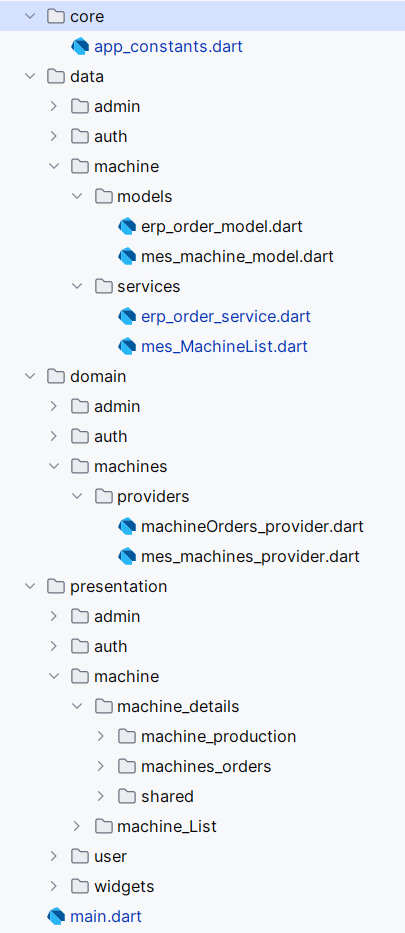
\includegraphics[width=\linewidth]{./media/MES_Sprint-2-Repport/screenshots/frontend-structure.png}
  \captionof{figure}{\techname{Flutter} machines domain --- layered architecture.}
  \label{fig:s2-flutter-architecture-s2}
\end{minipage}


5-second \texttt{Future.delayed} delay, emitting an updated list on every cycle and
yielding an empty list on error to prevent the \domainterm{StreamBuilder} from
entering an error state.


\modulename{ErpMachineOrdersService} (\modulename{erp\_order\_service.dart})
exposes three methods: \modulename{getMachineOrders} for fetching the order list,
\modulename{getStartOperationValidation} for triggering the start operation
endpoint and parsing the success/failure result, and
\modulename{fetchMachineOperationStatus} for retrieving active operation records.
A \modulename{streamMachines} generator on this service applies the same 5-second
polling pattern for the operations progress view.


\subsubsection{State Management Layer}

Two providers were introduced.
\modulename{MesMachinesProvider} (\modulename{mes\_machines\_provider.dart}) is a
plain (non-\texttt{ChangeNotifier}) provider that delegates directly to the
\modulename{MESMachineListService} stream. Because all state is carried by the
stream itself, no \texttt{notifyListeners} mechanism is needed and the
\domainterm{StreamBuilder} in the UI subscribes directly to the emitted values.

\modulename{MachineordersProvider} (\modulename{machineOrders\_provider.dart})
wraps both the order list fetching and the operation start flow with the standard
\texttt{ChangeNotifier} pattern. It exposes \modulename{getMachineOrders} which
populates a \modulename{machineOrders} list, and \modulename{startOrder} which
calls the service and returns a boolean success flag. It also exposes
\modulename{getMachineOperationsStatusStream} which passes the polling stream
through directly to the UI layer.

\subsubsection{User Interface}

The \uilabel{Machine List Page} is the entry point for operators after login. It
displays a live-updating grid (tablet/desktop) or list (mobile) of machine cards
scoped to the authenticated work centre. Each card shows the machine name, its
current status with a colour-coded badge, and the active production order number.
The layout adapts across breakpoints: a single-column list below 600 dp, a
two-column grid below 1024 dp, and a four-column grid above.
As illustrated in Figure~\ref{fig:s2-ui-machine-list}, the interface is consistent
across both desktop and mobile platforms.

\begin{figure}[H]
  \centering
  \setlength{\fboxsep}{5pt}
  \colorbox{black}{%
    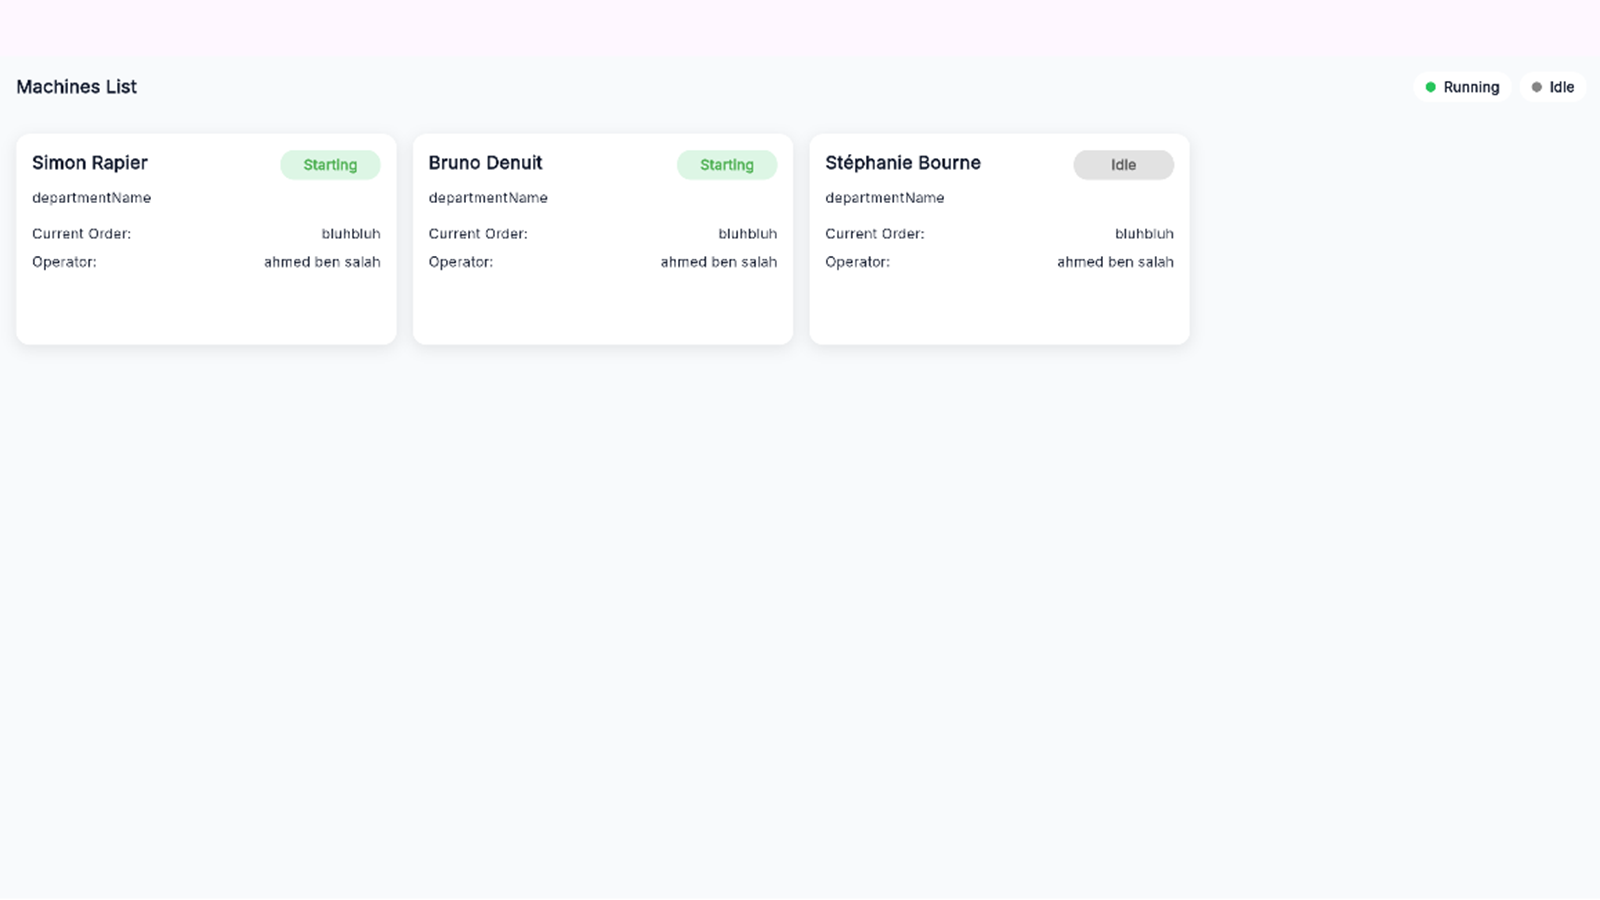
\includegraphics[height=0.3\textheight,keepaspectratio]{./media/MES_Sprint-2-Repport/UI/desktop-machines.png}%
    \hspace{\fboxsep}%
    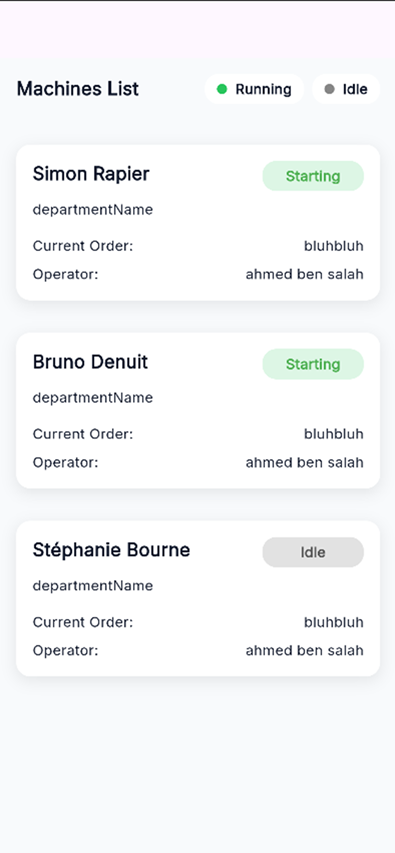
\includegraphics[height=0.3\textheight,keepaspectratio]{./media/MES_Sprint-2-Repport/UI/mobile-machines.png}%
  }
  \caption{\uilabel{Machine List Page} --- desktop and mobile views.}
  \label{fig:s2-ui-machine-list}
\end{figure}

The user interface for the machines domain is split across two top-level pages
accessible via a shared \uilabel{Top Navigation Bar} with tabs for
\uilabel{Orders}, \uilabel{Progress}, \uilabel{Consumable}, and \uilabel{History}.

The \uilabel{Machine Orders Page} displays the production routing lines assigned to the selected machine. A \uilabel{Global Search Bar} allows filtering by free text (order number, item description, or date), by status, and sorting by planned start date. Order cards use a responsive layout that switches between a stacked \domainterm{narrow layout} and a side-by-side \domainterm{wide layout} at a 520 dp breakpoint. Only \domainterm{Released} orders display an active \uilabel{Start Order} button; \domainterm{Planned} and \domainterm{Firm Planned} orders show it disabled. Figure~\ref{fig:s2-ui-machine-orders} illustrates both the desktop and mobile views.

\begin{figure}[H]
  \centering
  \setlength{\fboxsep}{5pt}
  \colorbox{black}{%
    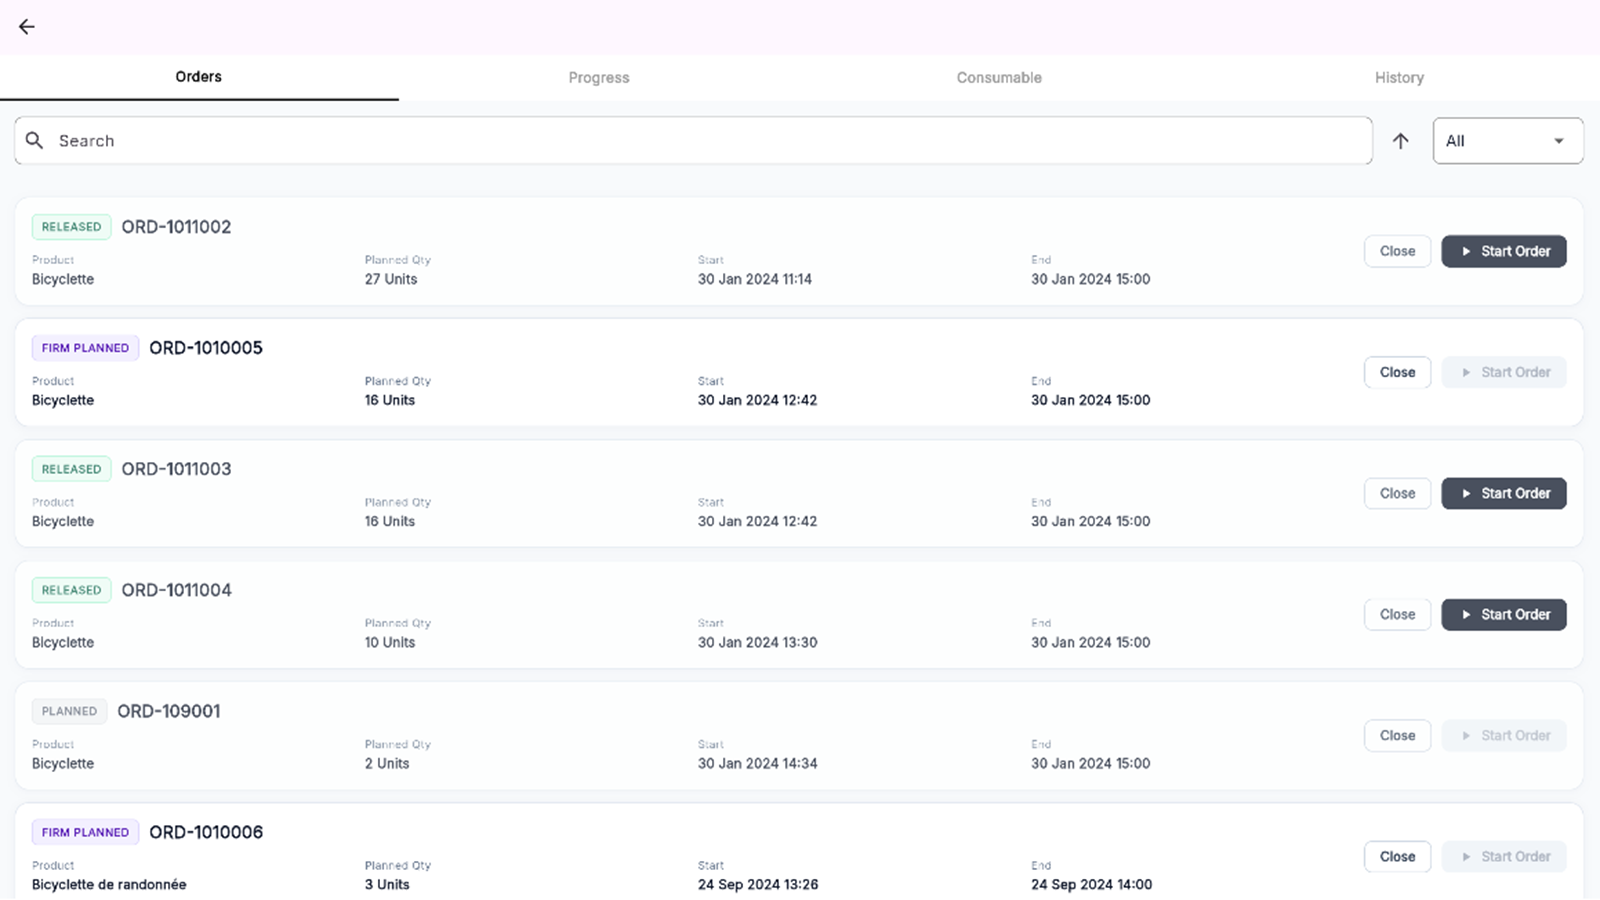
\includegraphics[height=0.3\textheight,keepaspectratio]{./media/MES_Sprint-2-Repport/UI/dektop-waiting_orders.png}%
    \hspace{\fboxsep}%
    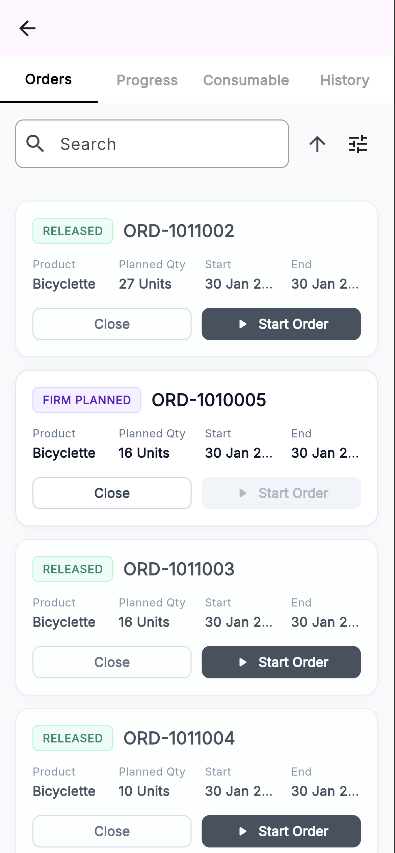
\includegraphics[height=0.3\textheight,keepaspectratio]{./media/MES_Sprint-2-Repport/UI/mobile-waiting_orders.png}%
  }
  \caption{\uilabel{Machine Orders Page} --- desktop and mobile views.}
  \label{fig:s2-ui-machine-orders}
\end{figure}

The \uilabel{Orders Progression Page} displays the currently active operations on
a machine, polling every 5 seconds. Each
operation card shows a colour-coded status badge (green for \domainterm{Running},
amber for \domainterm{Paused}), the order and operation identifiers, the last
updated timestamp, and a progress bar. The card layout also switches between narrow and wide
variants at the 520 dp breakpoint. \uilabel{Pause} and \uilabel{Resume} action
buttons adapt their colour and label to the current operation status, as shown in
Figure~\ref{fig:s2-ui-operations-progress}.

\begin{figure}[H]
  \centering
  \setlength{\fboxsep}{5pt}
  \colorbox{black}{%
    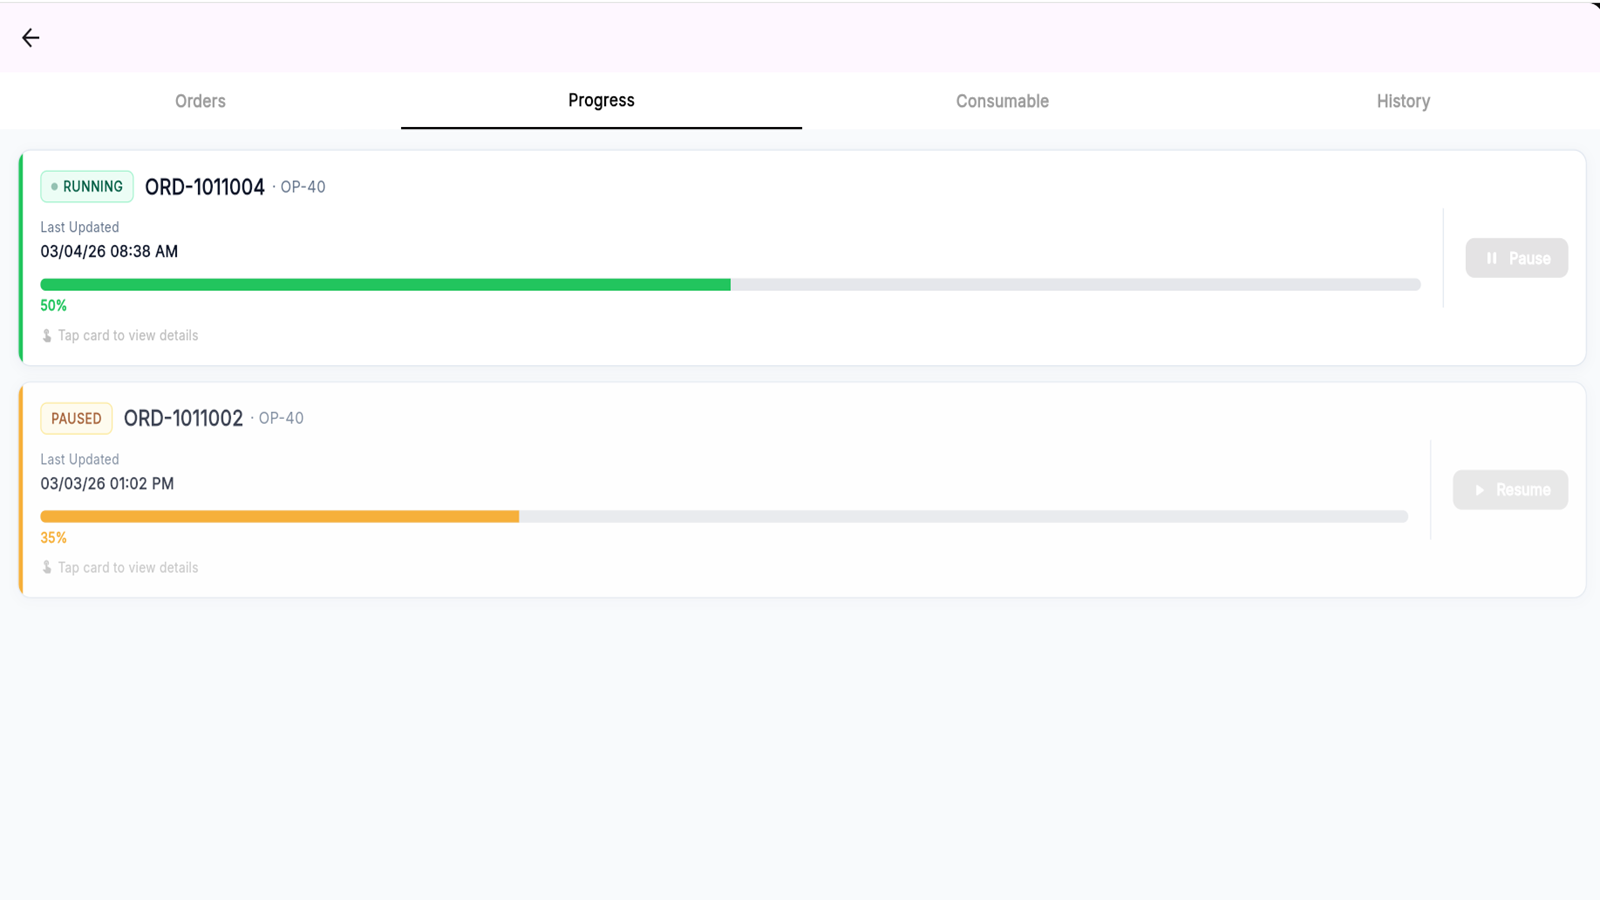
\includegraphics[height=0.3\textheight,keepaspectratio]{./media/MES_Sprint-2-Repport/UI/desktop-order_progress.png}%
    \hspace{\fboxsep}%
    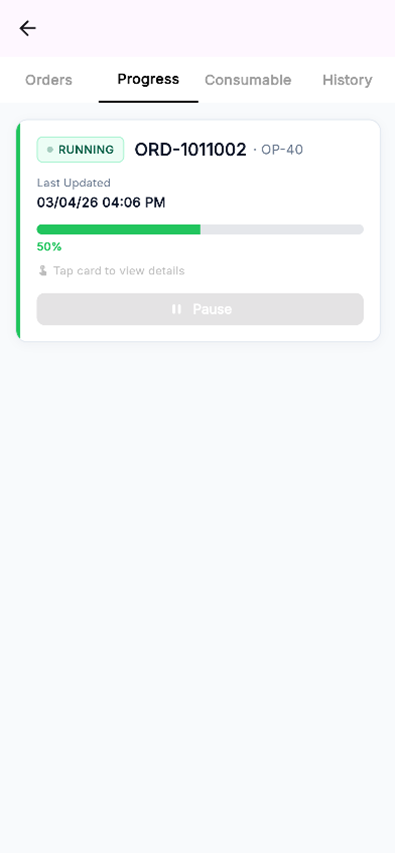
\includegraphics[height=0.3\textheight,keepaspectratio]{./media/MES_Sprint-2-Repport/UI/mobile-order_progress.png}%
  }
  \caption{\uilabel{Orders Progression Page} --- desktop and mobile views.}
  \label{fig:s2-ui-operations-progress}
\end{figure}

The \uilabel{Machine History Page} (Figure~\ref{fig:s2-ui-hist-page}) displays completed operations assigned to the selected machine, limited to \domainterm{Finished} and \domainterm{Cancelled} statuses. It shares the same layout and filtering behaviour as the \uilabel{Machine Orders Page} --- including free-text search, status filtering, and sort controls --- but omits the \uilabel{Start Order} button. Tapping an operation card navigates to its \uilabel{Operation Detail Page} for review. The \uilabel{Machine History Page} is accessible via the \domainterm{History} tab in the \techname{TopNavigationBar}. Figure~\ref{fig:s2-ui-hist-page} shows the desktop and mobile views.

\begin{figure}[H]
  \centering
  \setlength{\fboxsep}{5pt}
  \colorbox{black}{%
    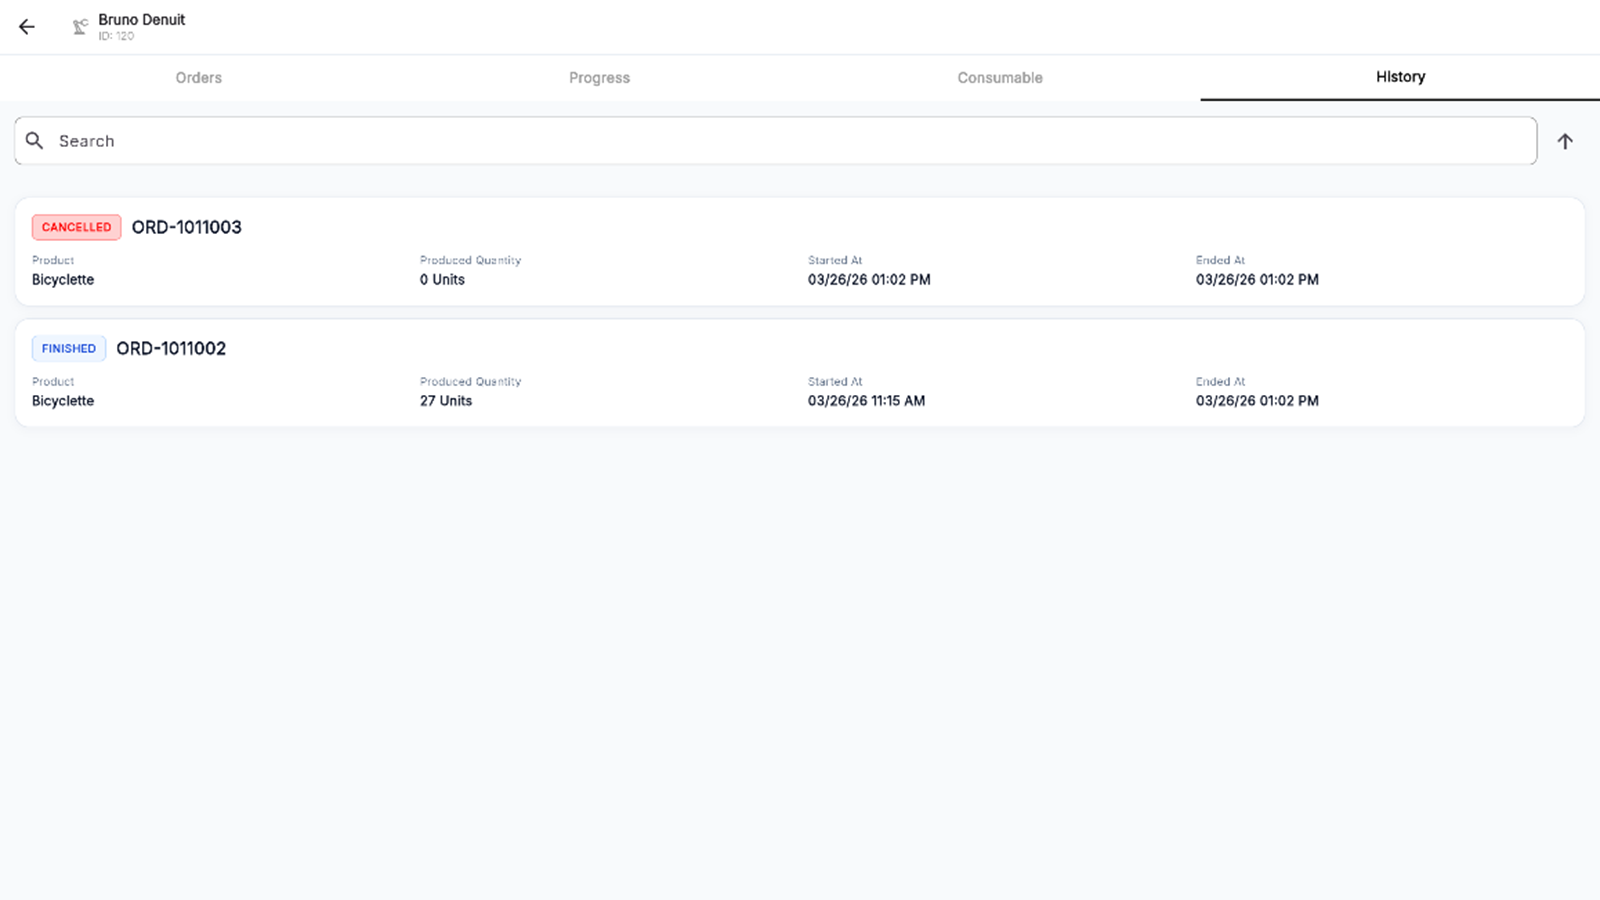
\includegraphics[height=0.3\textheight,keepaspectratio]{./media/MES_Sprint-2-Repport/UI/desktop-histPage.png}%
    \hspace{\fboxsep}%
    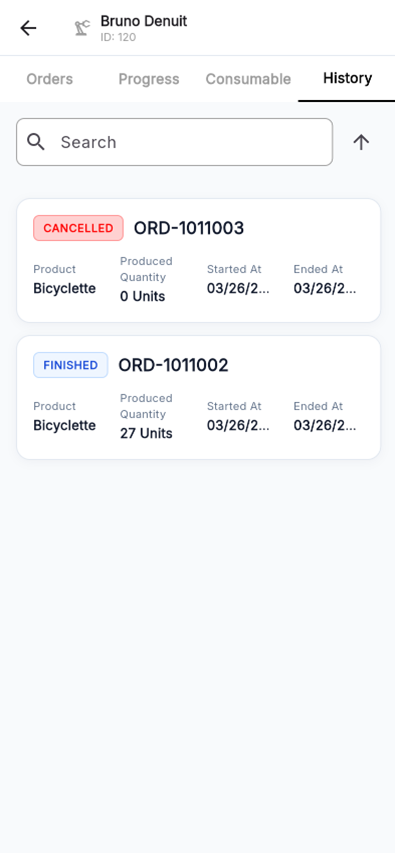
\includegraphics[height=0.3\textheight,keepaspectratio]{./media/MES_Sprint-2-Repport/UI/mobile-histPage.png}%
  }
  \caption{\uilabel{Machine History Page} --- desktop and mobile views.}
  \label{fig:s2-ui-hist-page}
\end{figure}


% ---------------------------------------------------------------------------
% CONCLUSION
% ---------------------------------------------------------------------------
\phantomsection
\section*{Conclusion}
\addcontentsline{toc}{section}{Conclusion}

This sprint successfully delivered the machine monitoring and production order
management foundation of the \domainterm{MES} application. On the backend, two
new append-only tables (\modulename{MES Machine Status} and
\modulename{MES Operation Status}) and a dedicated codeunit
(\modulename{MES Machine Actions}) were implemented in \techname{Business Central
  AL}, exposing four \domainterm{OData V4} endpoints that cover the full machine and
operation lifecycle. The append-only design ensures a complete, tamper-evident
audit trail of every state transition without requiring any record modification.

All business rules defined at the start of the sprint have been enforced: work
centre scoping (\businessrule{BR-MCH-002}), start operation validation
(\businessrule{BR-OPS-001}), immutable history (\businessrule{BR-OPS-002}),
active operation querying (\businessrule{BR-OPS-003}), and history scope
(\businessrule{BR-HIST-001}). The \techname{Flutter} frontend delivers a
responsive, real-time interface with 5-second polling streams for the machine
list and operations progress view, and a one-shot history load for the completed
operation audit log. The codebase is now ready to extend in Sprint~3 with
consumable tracking, operation finishing, and production declaration.
